\begin{enumerate}[\Large \bfseries 1.]

%----------1.
\item 

\begin{enumerate}[\bfseries a)]
    
    %----------a)
    \item \textbf{Análisis del problema.}\\
	
	Sea $x$ la entrada, entonces se podrá escoger entre:
	$$x=t \qquad o \qquad x=r \qquad o \qquad o x=c$$
	de donde se dibujara la figura correspondiente según el usuario haya elegido.\\
	Si $x$ es distinto a $t$ o $x$ o $c$ entonces se escribirá el mensaje de $"no\; v\mbox{á}lido"$
	Para poder graficar la orden dada se debe programar con turtle.\\\\

    %----------b)
    \item \textbf{Diagrama de flujo.}\\
	\begin{center}
	    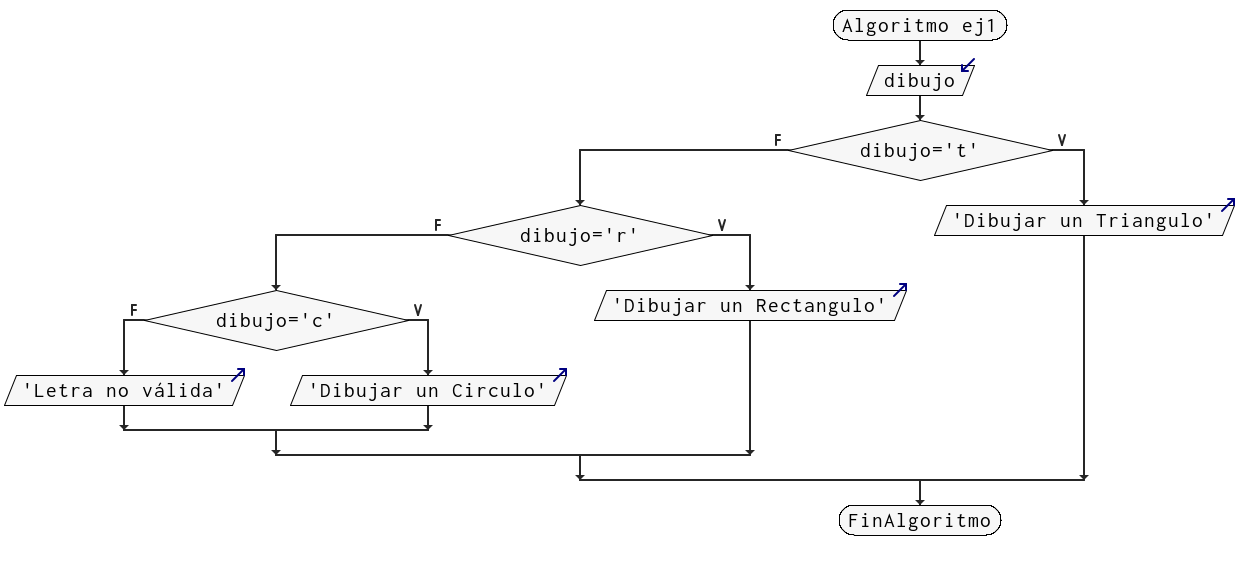
\includegraphics[scale=.37]{imagenes/tarea4/ej1.png}
	\end{center}

    %----------c)
    \item \textbf{Prueba de escritorio.}\\
	\begin{center}
	    \begin{tabular}{c|c}
		Dibujo&Print\\
		\hline
		t&Dibujar un triangulo\\
		\hline
		r&Dibujar un rectángulo\\
		\hline
		c&Dibujar un Circulo\\
	    \end{tabular}
	\end{center}
	\vspace{4cm}
    
    %----------d)
    \item \textbf{Código fuente.}\\ 
	
	\lstinputlisting[language=Python]{python/tarea4/ej1.py}
	\vspace{3cm}
    
    %----------e)
    \item \textbf{Prueba de la ejecución del programa}.\\
	\begin{center}
	    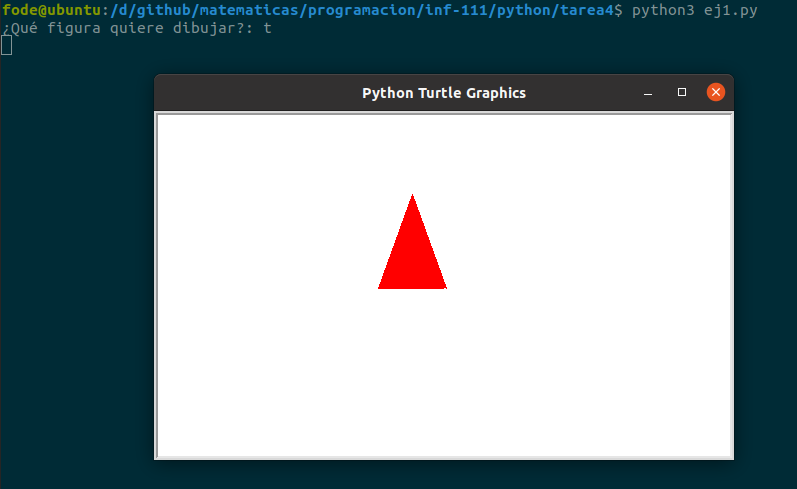
\includegraphics[scale=.5]{imagenes/tarea4/ej1_1.png}
	    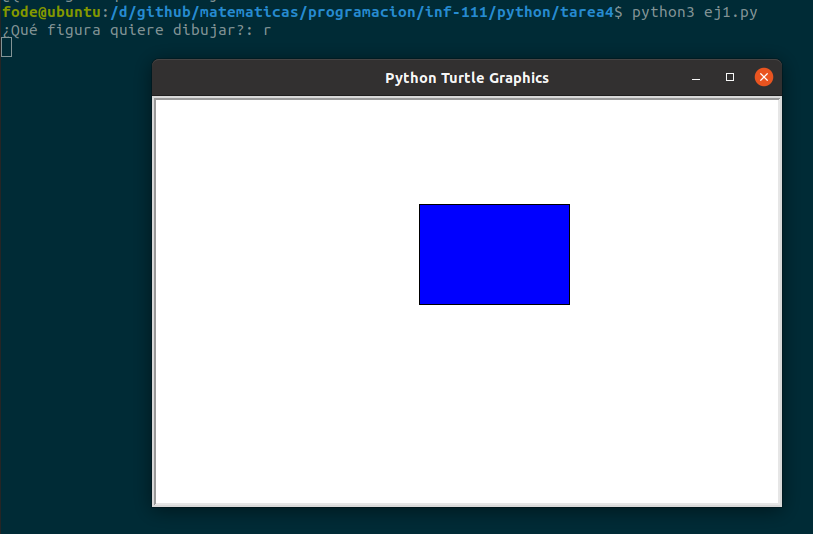
\includegraphics[scale=.5]{imagenes/tarea4/ej1_2.png}
	    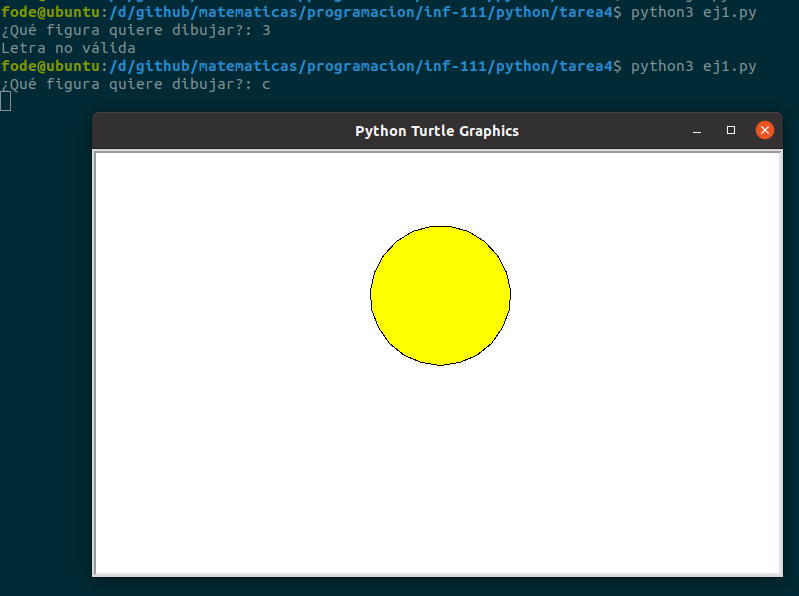
\includegraphics[scale=.5]{imagenes/tarea4/ej1_3.png}
	\end{center}

\end{enumerate}

\newpage

%----------2.
\item 

\begin{enumerate}[\bfseries a)]
    
    %----------a)
    \item \textbf{Análisis del problema.}\\


    %----------b)
    \item \textbf{Diagrama de flujo.}\\
	\begin{center}
	    %\includegraphics[scale=.9]{imagenes/tarea4}
	\end{center}

    %----------c)
    \item \textbf{Prueba de escritorio.}\\
	\begin{center}
	    \begin{tabular}{c|c|c}
		r&h&v\\
		\hline
		2&3&12$\pi$\\
	    \end{tabular}
	\end{center}
	\vspace{1cm}
    
    %----------d)
    \item \textbf{Código fuente.}\\ 
	
	%\lstinputlisting[language=Python]{python/tarea4}
	\vspace{1cm}
    
    %----------e)
    \item \textbf{Prueba de la ejecución del programa}.\\
	\begin{center}
	    % \includegraphics[scale=.7]{imagenes/tarea4}
	\end{center}

\end{enumerate}

\newpage

\end{enumerate}
